\documentclass[a4paper]{article}

\usepackage[english]{babel}
\usepackage[utf8]{inputenc}
\usepackage{amsmath,amsfonts}
\usepackage{graphicx}
\usepackage[colorinlistoftodos]{todonotes}
\usepackage[margin=1in]{geometry}
\usepackage{enumitem}
\usepackage{multirow}
\usepackage{graphicx,wrapfig,lipsum}
\usepackage{graphicx} % for images
\usepackage{caption} % for captions under images/figures
\usepackage{url} % for urls


\setcounter{tocdepth}{5}
\setcounter{secnumdepth}{5}

\title{CS 669 Assignment 2}

\author{Rohit Patiyal \\ Devang Bacharwar \\ Mani Kumar}

\date{\today}

\begin{document}


\maketitle

\vspace{2.0cm}

\tableofcontents

\clearpage

\section {Objective}
	
	\begin{enumerate}
		\item{
Build Bayes classifier using K-nearest neighbour method for class-conditional density estimation using DTW distance. }
			
		\item{Build Bayes classifier using Discrete HMM (DHMM).}
	\end{enumerate}
	
		
\vspace{1.0cm}

\section{Procedure for kNN classifier with DTW}
	\begin{enumerate}
	  \item {Data for each class is partitioned into 75 \% for training (class labels are known to the classifier) and 25
	  \% for testing (class labels are not known)}
	 
     \item {Labels for test data are calculated by varying different values of k $\epsilon$ \{ 1, 2, 3, $\cdots$ num of training patterns\} and accuracies for each k are calculated and plotted.}
     \item {
      DTW (Dynamic Time Warping) is used as the metric to compare the similarity of the test sample with the training data.     
     }
	 
	\end{enumerate}

\vspace{1.0cm}



\section{Observations  for kNN classifier with DTW}
	 
     \subsection{Image Scene Data Set} 
     
	
	\indent \par{	The Data set contains a total of 1112 samples out of which 833 are partitioned to be training samples and 279 as test samples.}
        \par{Each test sample is a fixed sized (36) sequence of feature vectors each having fixed number of dimensions(23).}
      	\par{The Data set consists of three classes Forest, Mountain and Open Country.} 
        
     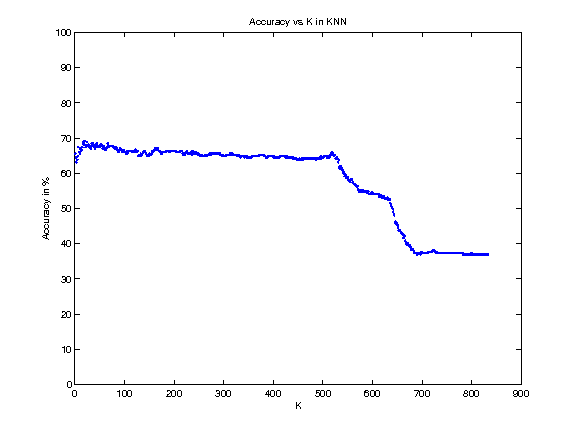
\includegraphics[width=\textwidth]{accScene.png}
		  	\captionof{figure}{ Accuracy vs number of nearest neighbours considered in kNN} % [4]
     	
        
        
        Here we can see that the accuracy tends to better when K (number of neighbours) considered for deciding the label are around 20-550 which gives accuracies around 65-70 \%.
 \subsection{Spoken Digit Data Set} 
       
       \indent \par{	The Data set contains a total of 480 samples out of which 360 are partitioned to be training samples and 120 as test samples.}
        \par{Each test sample is a varied sized sequence of feature vectors each having fixed number of dimensions(39).}
      	      
       \includegraphics[width=\textwidth]{accsd.png}
		  	\captionof{figure}{ Accuracy vs number of nearest neighbours considered in kNN} % [4]
     	
        
        
              Here we can see that the accuracy tends to better when K (number of neighbours) considered for deciding the label are around 15-200 which gives accuracies around 95-100 \%.
         

\section{Procedure for Discrete HMM based bayes classifier}
	\begin{enumerate}
	  \item {Data for each class is partitioned into 75 \% for training (class labels are known to the classifier) and 25 \% for testing (class labels are not known)}
     \item {Labels for test data are calculated by varying different values of k $\epsilon$ \{ 1, 2, 3, $\cdots$ num of training patterns\} and accuracies for each k are calculated and plotted.}
     \item {
      DTW (Dynamic Time Warping) is used as the metric to compare the similarity of the test sample with the training data.     
     }
	 
	\end{enumerate}

\section{Observations for Discrete HMM based bayes classifier}
	 
     \subsection{Image Scene Data Set} 

	     \subsubsection{64 clusters components}
         \begin{center}
		\vspace{10pt} % [3]
			Correct   : 234	\\
			Incorrect : 45	\\
			Accuracy  : 83.87 \\
		
			\begin{tabular}{ |c|c|c|c|c| }
			\hline
			& & \multicolumn{3}{| c |}{Predicted} \\
			\hline
			& & Class 1 & Class 2 & Class 3\\
			\hline
			\multirow{3}{*}{\rotatebox[origin=c]{90}{Act.}} & Class 1 & 65 & 10 & 7\\
			& Class 2 & 2 & 85 & 7\\
			& Class 3 & 3 & 16 & 84\\
			\hline
			\end{tabular}
			\end{center}

	 \subsection{Spoken Digit Data Set} 

     \subsubsection{64 clusters components}
         \begin{center}
		\vspace{10pt} % [3]
			Correct   : 234	\\
			Incorrect : 45	\\
			Accuracy  : 83.87 \\
		
			\begin{tabular}{ |c|c|c|c|c| }
			\hline
			& & \multicolumn{3}{| c |}{Predicted} \\
			\hline
			& & Class 1 & Class 2 & Class 3\\
			\hline
			\multirow{3}{*}{\rotatebox[origin=c]{90}{Act.}} & Class 1 & 65 & 10 & 7\\
			& Class 2 & 2 & 85 & 7\\
			& Class 3 & 3 & 16 & 84\\
			\hline
			\end{tabular}
			\end{center}

\section{Conclusion}
	As per the observations, we can make the following conclusions :
	
	\begin{enumerate}
	  \item Different results are obtained when number of nearest neighbours $k$ are varied.   	
	  
      \item The spoken digit is better classified by the kNN and DTW based bayes classifier.  
	\end{enumerate}
    \center{          
\ldots{}    
}
\end{document}

            